\begin{frame}
  \titlepage
  \centering
  
\includegraphics[scale=.4]{assets/logo/eurecom.png}

\end{frame}


\begin{frame}{Before Starting: a collaborative effort!}
    \centering
    
    % --- Row 1 ---
    \begin{columns}[t] % [t] ensures top alignment if names have different lengths
        
        % Collaborator 1
        \begin{column}{0.3\textwidth}
            \centering
            % Replace 'example-image-a' with your filename (e.g., 'john.jpg')
            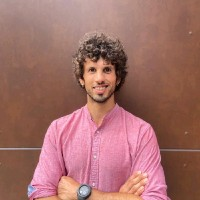
\includegraphics[width=0.8\linewidth]{pics/franzese.jpg}
            \par\vspace{5pt}
            \textbf{Giulio Franzese}\\
        \end{column}
        
        % Collaborator 2
        \begin{column}{0.3\textwidth}
            \centering
            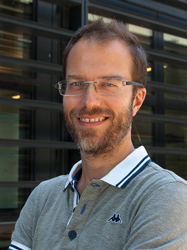
\includegraphics[width=0.7\linewidth]{pics/michiardi-pietro_1.jpg}
            \par\vspace{5pt}
            \textbf{Pietro Michiardi}\\
        \end{column}
        
        % Collaborator 3
        \begin{column}{0.3\textwidth}
            \centering8
            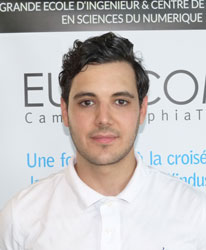
\includegraphics[width=0.8\linewidth]{pics/bounoua-mustapha.jpg}
            \par\vspace{5pt}
            \textbf{Bounoua Mustapha}\\
        \end{column}
        
    \end{columns}
    
    %\vspace{1cm} % Space between rows
    
    % --- Row 2 ---
    \begin{columns}[t]
        
        % Collaborator 4
        \begin{column}{0.3\textwidth}
            \centering
            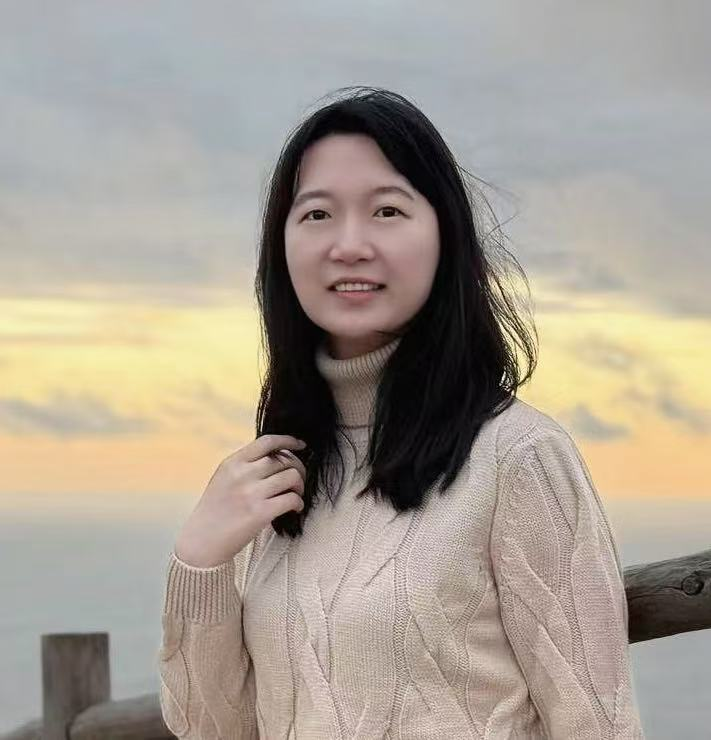
\includegraphics[width=0.8\linewidth]{pics/headshot_chao (1).jpg}
            \par\vspace{5pt}
            \textbf{Chao Wang}\\
        \end{column}
        
        % Collaborator 5
        \begin{column}{0.3\textwidth}
            \centering
            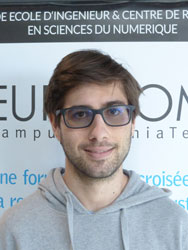
\includegraphics[width=0.7\linewidth]{pics/foresti-alberto.jpg}
            \par\vspace{5pt}
            \textbf{Alberto Foresti}\\
        \end{column}
        
        % Collaborator 6
        \begin{column}{0.3\textwidth}
            \centering
            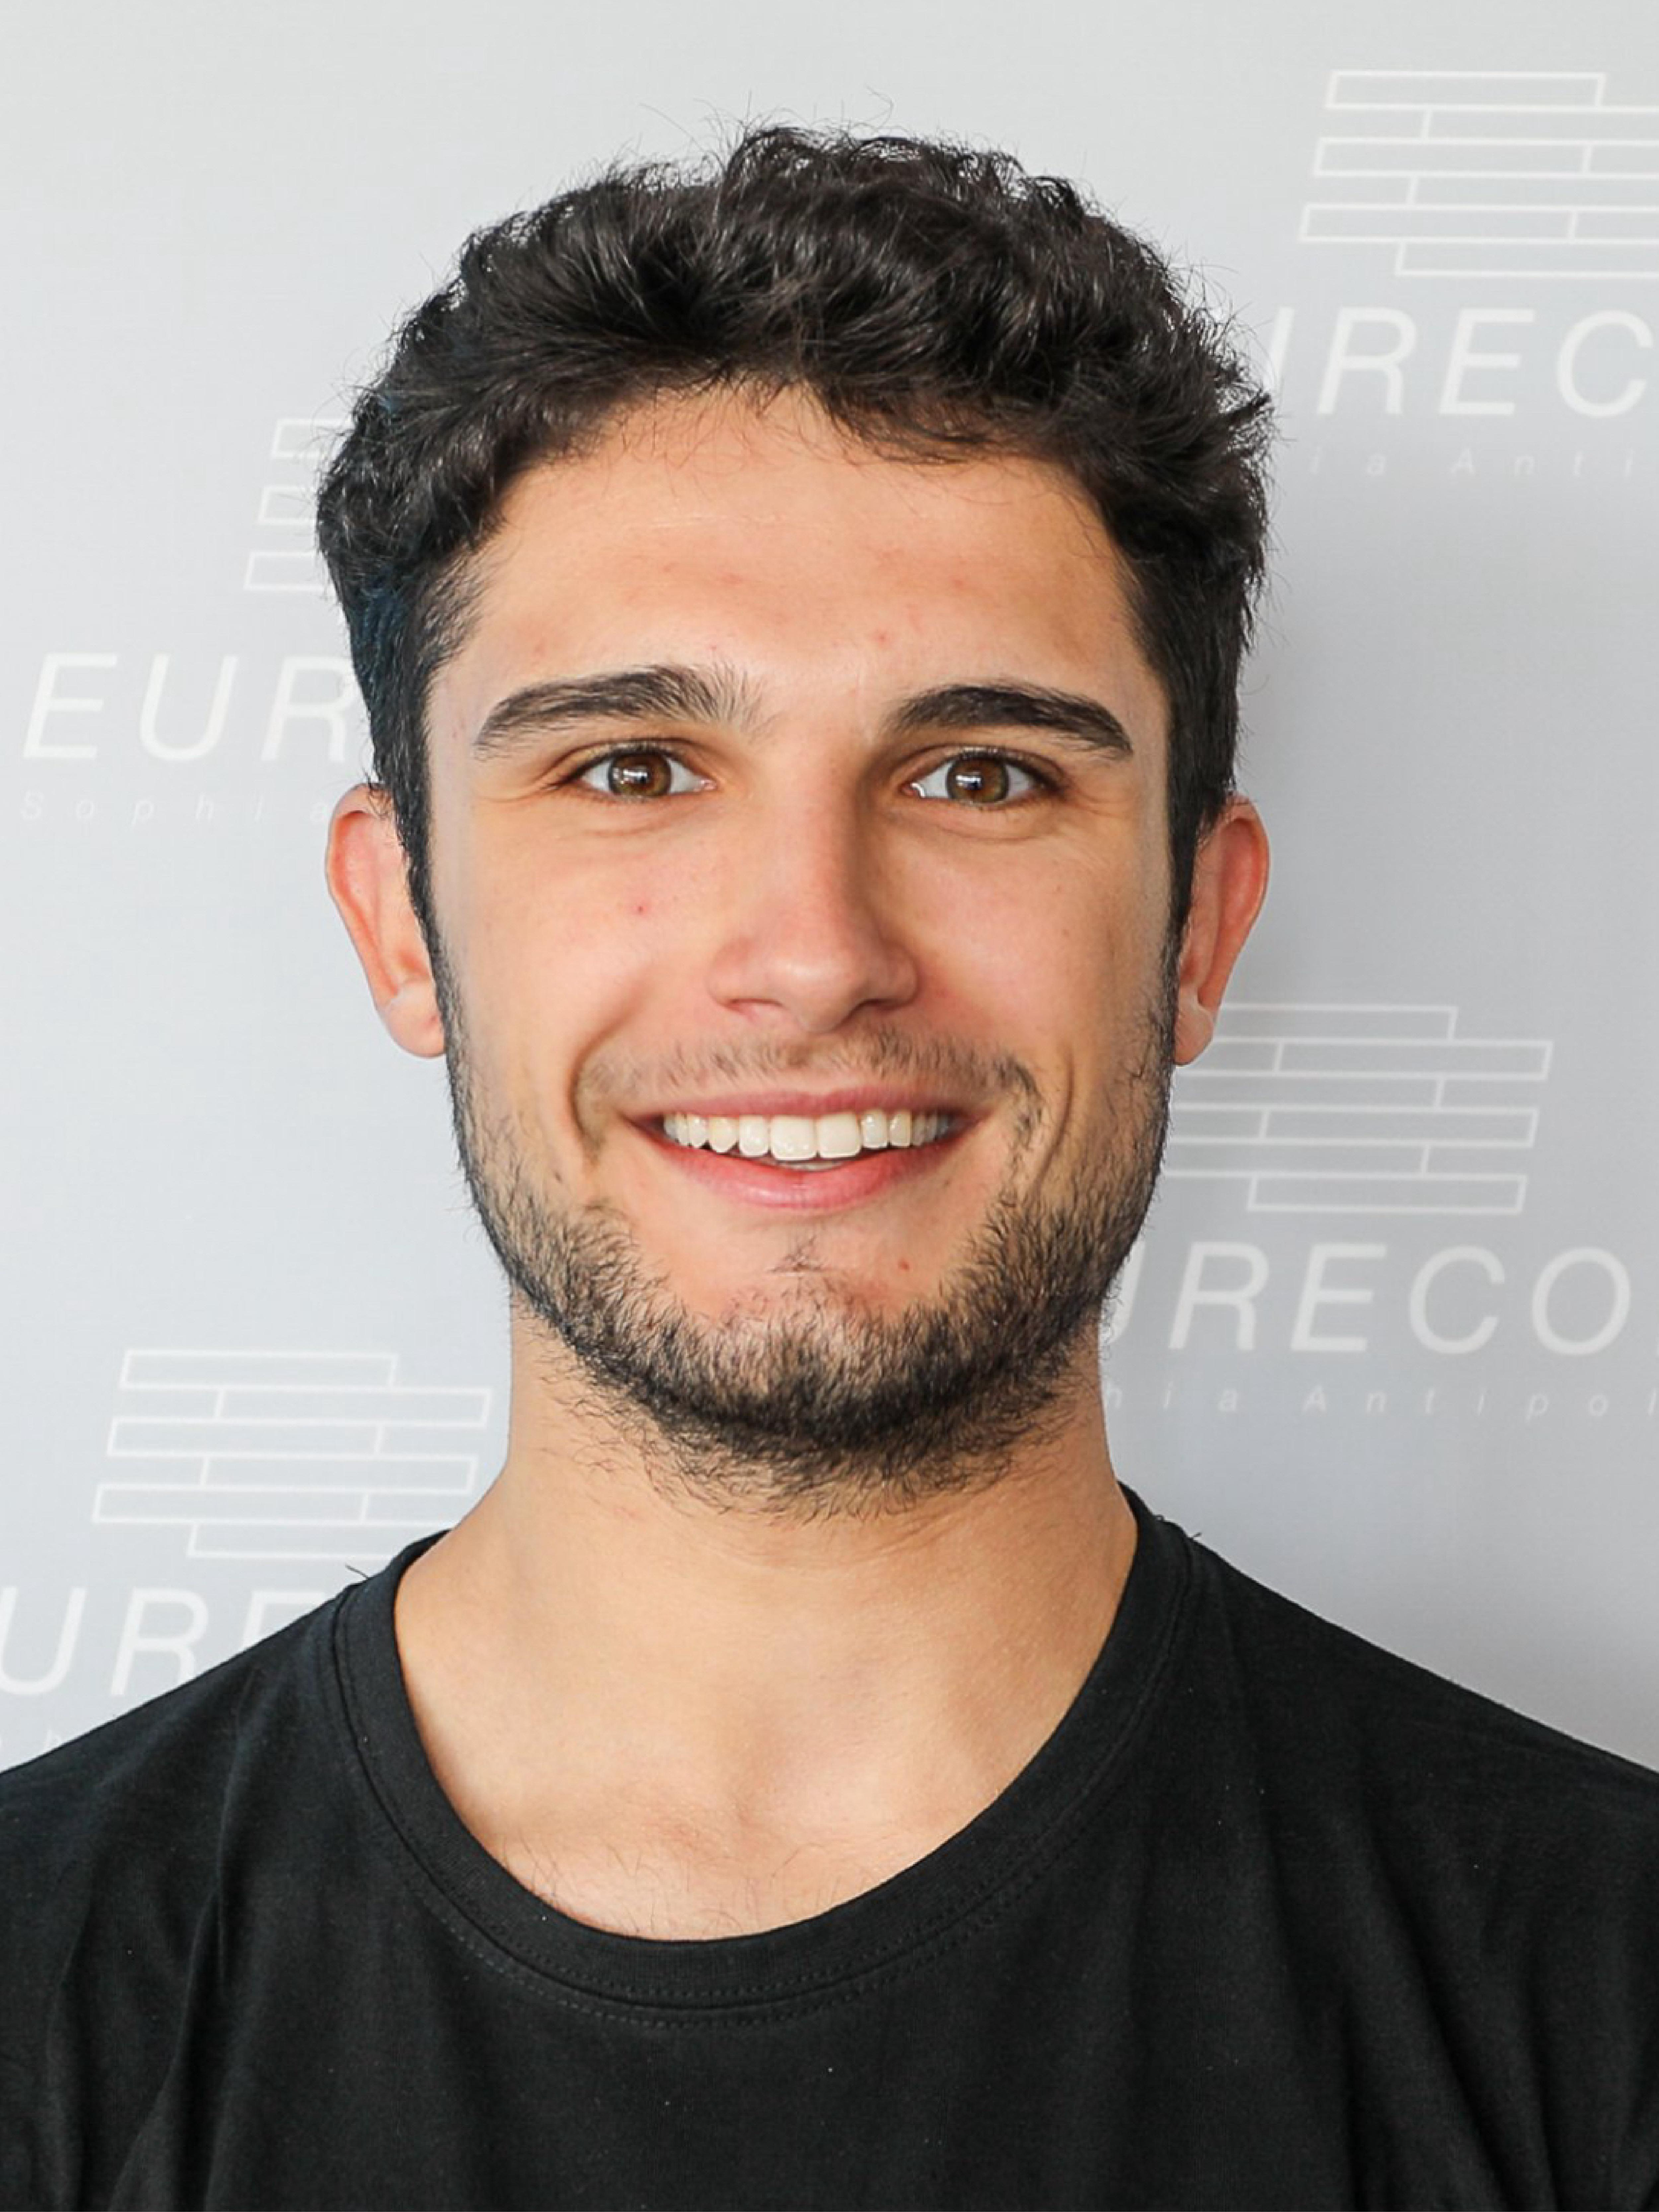
\includegraphics[width=0.7\linewidth]{pics/nepote-luca.jpg}
            \par\vspace{5pt}
            \textbf{Luca Nepote}\\
        \end{column}
        
    \end{columns}
\end{frame}

%\begin{frame}{Outline}
%  \tableofcontents
%\end{frame}
\begin{frame}[allowframebreaks]{Summary of the Talk}
Spoiler of the talk:
\begin{itemize}
    \item How to compute MI leveraging particular families of diffusion processes
    \item Hints about generalisation using other class of processes (Discrete state spaces, Infinite dimensional spaces)
    \end{itemize}

    
Focus on applications! Generalisation of the MI to the cases of
\begin{itemize}
    \item Multivariate scenario (O-Information)
    \item Transfer Entropy for dynamical systems
\end{itemize}
\end{frame}


\part{Introduction}
\section{Mutual Information}

\begin{frame}[allowframebreaks]{Definition of Mutual Information}
  
  The mutual information between two random variables $X$ and $Y$ (or stochastic processes) is defined as:
  \begin{equation}
    \textsc{I}(X; Y) = \mathbb{E} \left[ \log \frac{d\mu^{X,Y}}{d\mu^X d\mu^Y} \right]
  \end{equation}
  where:
  \begin{itemize}
    \item $\mu^{X,Y}$ is the joint probability \textbf{measure} of $X$ and $Y$.
    \item $\mu^X$ and $\mu^Y$ are the marginal measures.
  \end{itemize}
The same definition holds when $X$ and $Y$ are stochastic processes.

\framebreak



\end{frame}


\begin{frame}{Mutual Information as a Fundamental Measure}
  
  \begin{itemize}
    \item Mutual information is a fundamental measure of statistical dependence between random variables.
    \item Imagine an omnipotent Daemon observing streams of data: \textbf{either} from the joint distribution $\mu^{X,Y}$ \textbf{or} from the product of the marginals $\mu^X \mu^Y$.
    \item Mutual information quantifies the rate at which the daemon can distinguish between these two cases.
    \item In practical terms:
    \begin{itemize}
      \item For discrete random variables, mutual information provides fundamental bounds on classification accuracy.
      \item For continuous variables, it sets limits on estimation variance.
    \end{itemize}
  \end{itemize}
\end{frame}

\begin{frame}{Interpretation of Mutual Information}
  
  \begin{itemize}
    \item In a communication system, mutual information measures how much information about a message is retained after transmission through a noisy channel.
    \item Interesting ML applications (to name a few): Representation Learning, Information Bottleneck, Generative Models enhancements, Interpretability...
  \end{itemize}
\end{frame}



\begin{frame}{Some examples}

\begin{flalign*}
    &\textsc{I}(A;B)=\int_{\mathrm{R}^{N\times M}} p(x,y)\log\frac{p(x,y)}{p(x)p(y)}dxdy, \quad \mu^{A,B}(dx,dy)=p(x,y)dxdy\\
    &\textsc{I}(A;B)=\sum_{x,y\in \mathcal{X}\times \mathcal{Y}} p(x,y)\log\frac{p(x,y)}{p(x)p(y)}, \quad \mu^{A,B}(x,y)=p(x,y)
\end{flalign*}

Critically we rely on i) knowledge of the measures ii) capability of computing integral/sums in closed form. Examples: AWGN Channel, Discrete RVs with known distribution... 
\end{frame}
\begin{frame}{Technical Simplification}

To lighten up a bit the notation, we present results for \textit{generic} Kullback-Leibler divergences:

\begin{equation}
    \KL{\mu}{\rho}\defeq \int\phi(\frac{\dd\mu}{\dd\rho})\dd \rho,\quad \text{with}\quad \phi(x)=x\log(x)
\end{equation}

Trivial excercise: show that $\textsc{I}(A,B)=\KL{\mu^{A,B}}{\mu^{A}\mu^{B}}$
\end{frame}

\section{Existing estimators}
\begin{frame}[allowframebreaks]{Mutual Information Estimators...?}

More than 80 years of research in three sentences:
\begin{itemize}
    \item For Continuous RVs \textit{approximate} the distributions as Gaussian, Laplace (insert anything which gives easy to compute formulas) and compute MI,e.g.
    {\small \[p(x,y)\simeq \mathcal{N}(\mu,\begin{bmatrix}
        \Sigma_{XX} &\Sigma_{XY}\\\Sigma_{XY}^\top &\Sigma_{YY}
    \end{bmatrix}) \rightarrow \textsc{I}(X,Y)=\frac{1}{2}\log(\frac{\det(\Sigma_{YY})\det(\Sigma_{XX})}{\det(\Sigma)})\]}
    \item For Discrete random variables, estimate the histogram of joint occurrences from dataset $\{x_i,y_i\}_{i=1}^N, x_i,y_i\in \mathcal{X}$, store them in a large matrix, and compute
   {\small \[ \hat{H}=\frac{1}{N}\begin{bmatrix} \#(x_i=0,y_i=0) &\dots & \#(x_i=0,y_i=M) \\ \#(x_i=1,y_i=0) &\dots & \#(x_i=1,y_i=M)\\ \vdots \end{bmatrix}, \quad \hat{I}=\sum_{j,k}\hat{H}_{j,k}\log \hat{H}_{j,k}\]}
    \item Combine the approaches (binning, clustering prototypes,etc...)
\end{itemize}

\framebreak

\textbf{Problem}: classical estimators fail in high dimensional scenarios necessitating advanced estimation methods like neural estimators.

\begin{itemize}


\item Two main families of neural approaches\begin{itemize}
    \item Discriminative: a classifier distinguish between samples from the joint ($\sim \mu^{A,B}$) or product of marginals ($\mu^A \mu^B$)
    \item Generative (likelihood based): fit parametrically $\mu^{A,B}$ and estimate MI using Montecarlo Methods
\end{itemize}
\item \textbf{Problem:} many existing neural estimators fail on challenging (long-tailed distrubutions) and not pass \textit{consistency tests}.
    \end{itemize}

\framebreak

Discriminative approaches in one slide (convex duality of $\phi(\cdot)$):

\[\phi^{*}(y)=\sup_{x}(xy-\phi(x)),\quad \phi^{**}(x)= \sup_{y}(yx-\phi^{*}(y)),\quad \phi^{**}(x)=\phi(x) \]

\begin{itemize}
    \item Donsker-Varahdan Thm:\begin{equation*}
        \KL{\mu}{\chi}=\sup_{T:\Omega\rightarrow\mathrm{R}}\E_\mu[T]-\log \E_\chi [\exp(T)]
    \end{equation*}
    \item From all possible functions $T$ to the smaller class of \textit{neural networks}:\[\sup_{T:\Omega\rightarrow\mathrm{R}}(\E_\mu[T]-\log \E_\chi [\exp(T)])\geq \sup_{\theta\in \mathrm{R}^K}(\E_\mu[T^\theta]-\log \E_\chi [\exp(T^\theta)]) \]



    \begin{figure}
        \centering
        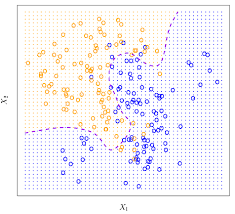
\includegraphics[width=0.5\linewidth]{figures/dec_bound.png}
        \label{fig:placeholder}
    \end{figure}
    \item \textbf{Big problems}: i) Good luck with MC estimation of $\log \E [\exp(T^\theta)]$ ii) For tail events estimation unreliable.
\end{itemize}
    \end{frame}

\part{Estimation via Diffusion}

\section{MINDE}

\begin{frame}[allowframebreaks]{Introduction}
\begin{itemize}
    \item Consider a generic random variable $A$ with probability measure $\mu^A$
    \item Build a simple SDE in $[0,T]$ with initial conditions $\sim \mu^A$
    \begin{equation}\label{eq:diffsdes}
    \begin{cases}
    \dd X_t=-X_t\dd t+\sqrt{2}\dd W_t,\\
    X_0=A\sim \mu^A
    \end{cases}
    \end{equation}
    where $W_t$ is a Brownian motion. \textbf{Informally}, $\dd W_t\sim \mathcal{N}(0,\dd t)$
    \item For engineers/physicists:
    \begin{equation}\label{eq:diffsdes_s}
    \frac{\dd X_t}{\dd t}=-X_t+\sqrt{2}\underbrace{\frac{\dd W_t}{\dd t}}_{N_t,\text{White Noise}}
    \end{equation}
    (even simpler: $X_t=h_t\star N_t$). We need measure theory and stoch. integrals for nonlinear drifts, etc...


    \item This SDE corresponds to a path measure $\mathbb{P}^{A}$ (\textbf{informally} events like $\text{Pr}(X_{0\leq t\leq T}\in \mathcal{S})$). 

\framebreak

\item Two SDEs which differ only by initial conditions have KL divergence 

\begin{equation}
 \KL{\mathbb{P}^{A}}{\mathbb{P}^{B}}=\E_{\mathbb{P}^{A}}\left[\log\frac{\dd\mathbb{P}^{A}}{\dd\mathbb{P}^{B}}\right]=\E_{\mathbb{P}^{A}}\left[\log\frac{\dd \mu^{A}}{\dd p^{B}}\right]=\KL{\mu^A}{\mu^B}  
\end{equation}
\item Disintegration of measures explains why (simply Markov): \[\frac{\dd {P}^{A}}{\dd {P}^{B}}=\frac{\dd \left(\mathbb{P}^{A}\#_{X_{0}}\right)}{\dd \left(\mathbb{P}^{B}\#_{X_{0}}\right)}\frac{\dd \mu^A(X_{0})}{\dd \mu^B(X_{0})}=\frac{\dd \mu^A(X_{0})}{\dd \mu^B(X_{0})}\]
\end{itemize}  
\framebreak
\textbf{Time-reversal} $\hat{X}_t\defeq X_{T-t}$:
\begin{itemize}
    \item KL between path measures is invariant to time-reversal $\KL{\mathbb{P}^{A}}{\mathbb{P}^{B}}=\KL{\hat{\mathbb{P}}^{A}}{\hat{\mathbb{P}}^{B}}$
    \item Time reversal of SDE is again an SDE (provided technical conditions [ Leonard 2014])
    \begin{equation}
         \dd \hat X_t=\hat X_t+2 \underbrace{\nabla\log \frac{\dd\mu_{T-t}^A}{\dd x}(\hat X_t)}_{\text{score function!}}\dd t+ \sqrt{2}\dd \hat W_t
    \end{equation}
    with $\dd x$ the Lebesgue measure
    \item Score function $\leftrightarrow$ Denoiser: \begin{equation}
        \nabla\log \frac{\dd\mu_t^A}{\dd x}(x)=\nabla\log p^A_t(x)=\frac{ \exp(-t){\color{red}\E_{{\mathbb{P}^{A}}}[X_0\g X_t=x]}-x}{1-\exp(-2t)}
    \end{equation}
\end{itemize}


\framebreak
\textbf{Girsanov theorem}: (informal) express the KL between path measures corresponding to two \glspl{SDE} with different drifts.

\begin{equation}
 \KL{\hat{\mathbb{P}}^{A}}{\hat{\mathbb{P}}^{B}}\simeq  \E_{   {\mathbb{P}}^{\mu^A}}\left[\int\limits_0^T\norm{\nabla\log p^{A}_t(X_t)-\nabla\log p^{B}_t(X_t) }^2\dd t\right]
\end{equation}
\begin{itemize}
    \item Combining with $\KL{\mathbb{P}^{A}}{\mathbb{P}^{B}}=\KL{\hat{\mathbb{P}}^{A}}{\hat{\mathbb{P}}^{B}}$ we can obtain a KL-estimator!
\end{itemize}




\framebreak

... but do we know the score? In general, no.

Solution$\rightarrow$ parametric denoiser (score network)
\begin{equation}
    \mathcal{L}(\theta)=\E[\norm{\text{net}_\theta(X_t,t)-X_0}^2]
\end{equation}
Remember $X_0=A$. Basically a self-supervised procedure
\begin{itemize}
    \item Start with a dataset.
    \item Corrupt it with various level of noise.
    \item Try to learn a proper denoiser.
\end{itemize}

   
\end{frame}
\begin{frame}{Score-based Generative models?}
The time reversal of diffusion processes is currently one of the main ingredients behind the extremely popular generative models!
\begin{figure}
    \centering
    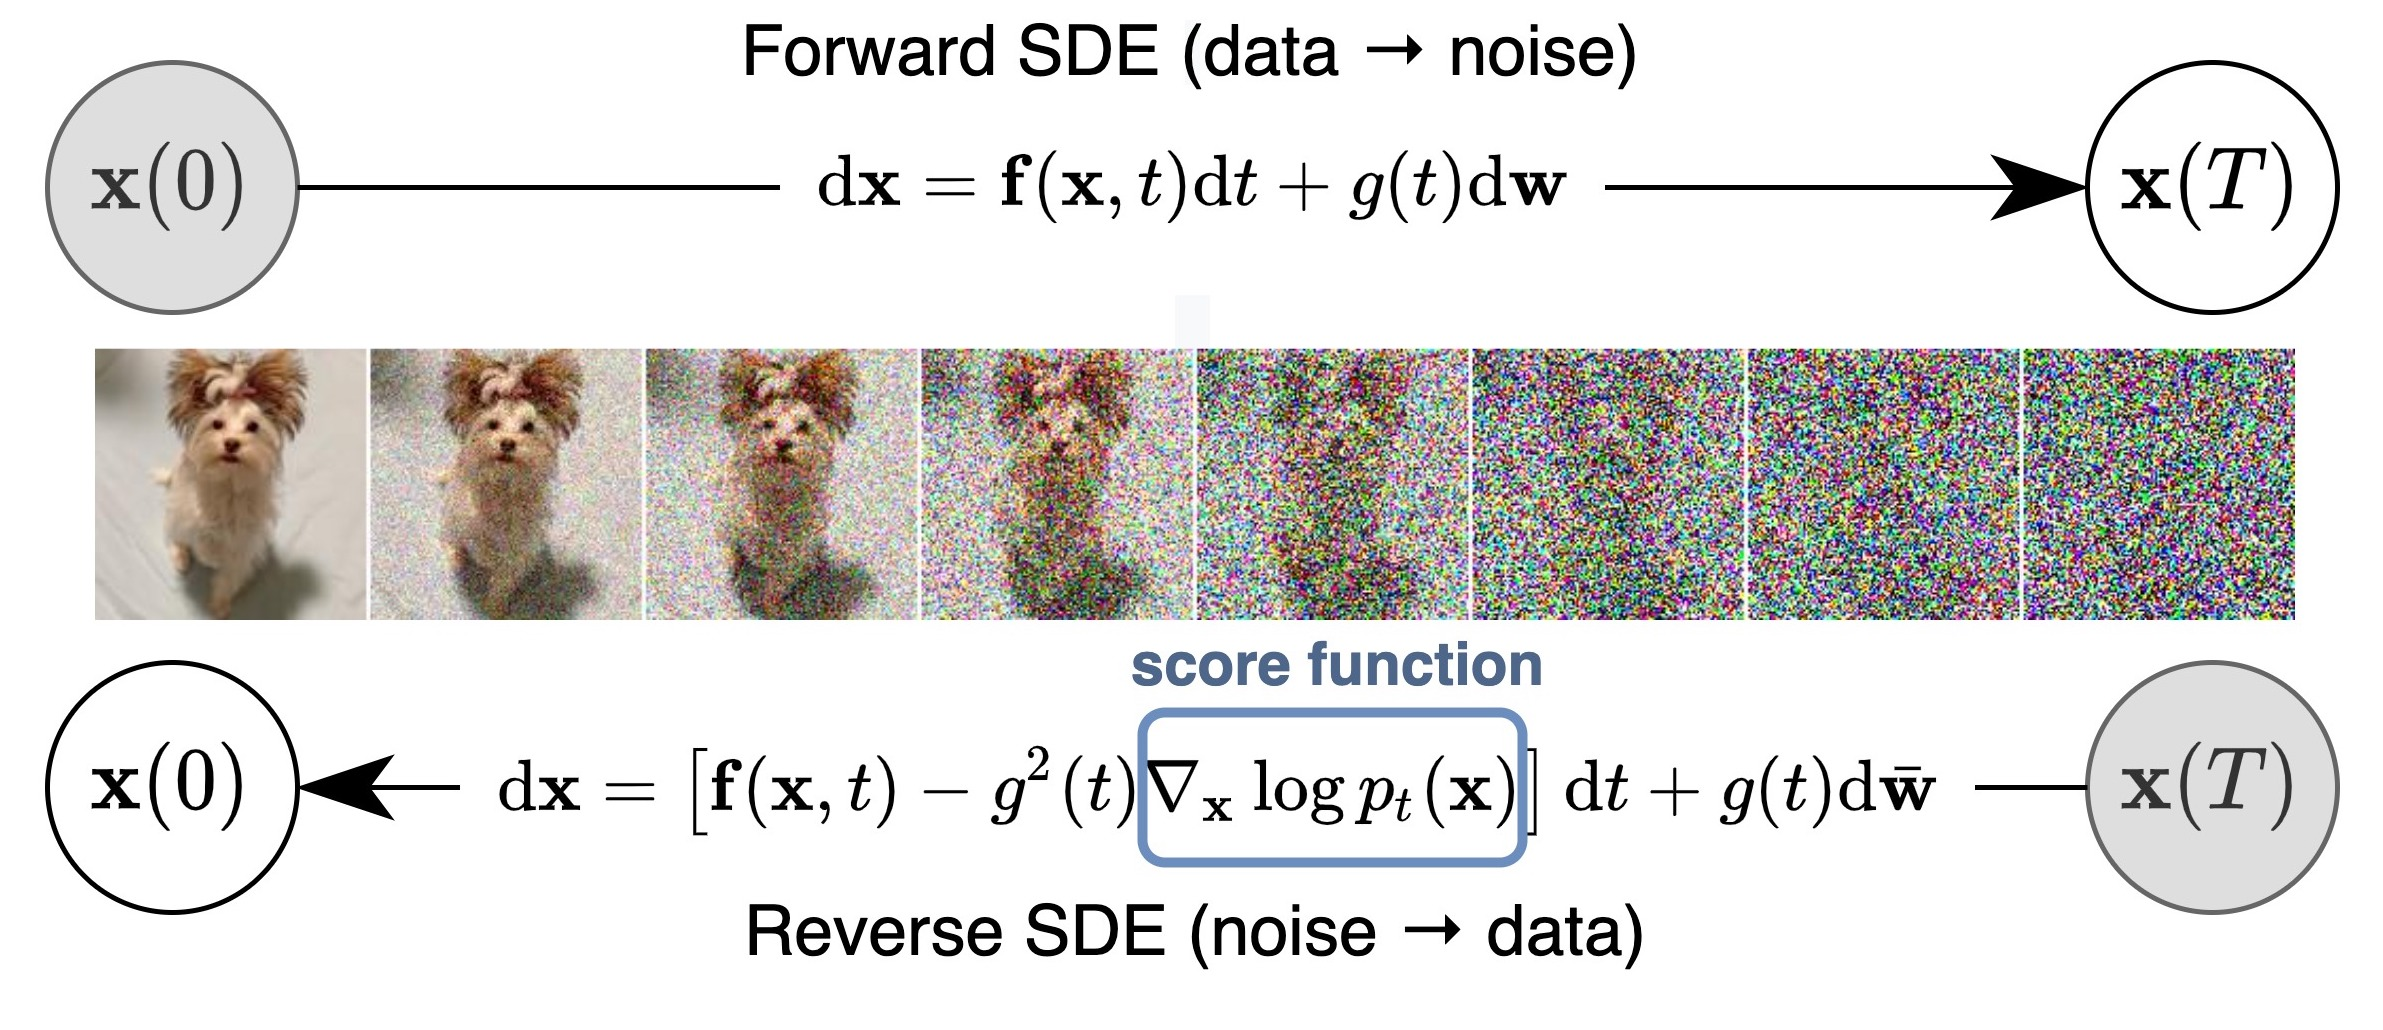
\includegraphics[width=0.8\linewidth]{figures/sde_schematic.jpg}
    \caption{Song et al. "Score-Based Generative Modeling through SDEs"}
\end{figure}
    
\end{frame}

%\section{Variational Approach to Score-based Models}
\begin{frame}{Mutual Information Neural Diffusion Estimation}
Mutual Information between two random variables $A,B$ (many equivalent formulations):
\begin{equation}
\textsc{I}(A,B)=\KL{\mu^{A,B}}{\mu^A\mu^B}    
\end{equation}
Idea: estimation using score functions!
Two families of diffusion processes: joint (J) and conditional (C).
\begin{flalign*}
   & \begin{cases}
    \dd \left[X_t,Y_t\right]^\top =-[X_t,Y_t]^\top \dd t+ \sqrt{2}\left[\dd W_t,\dd W'_t\right]^\top\\
    [X_0,Y_0]^\top\sim \mu^{A,B}
    \end{cases}\\&
    \begin{cases}
        \dd X_t=-X_t\dd t+\sqrt{2}\dd W_t \\
        X_0\sim \mu^{A\g B}
    \end{cases}
\end{flalign*}

\end{frame}

%\section{KL Divergence and Score Functions}
\begin{frame}[allowframebreaks]{Mutual Information Neural Diffusion Estimation}
First family, MINDE-C:
\begin{algorithm}[H]
\caption{Estimate Mutual Information using Diffusion Models}
\begin{algorithmic}[1]
\State $[A, B] \sim \mu^{A,B}$ \Comment{Sample from joint distribution}
\State $t \sim \mathcal{U}[0, T]$ \Comment{Uniformly sample $t$ from $[0, T]$}
\State $X_t \gets \exp(-t)A + \sqrt{1-\exp(-2t)} \epsilon$, where $\epsilon \sim \mathcal{N}(\zerovect,\eye)$ \Comment{Simulate diffusion}
\State ${s}^{A} \gets \text{net}_\theta([X_t, 0], t, c = 0)$ \Comment{Compute unconditional score using network $\text{net}_\theta$}
\State $s^{A_{B}} \gets \text{net}_\theta([X_t, B], t, c = 1)$ \Comment{Compute conditional score}
\State $\hat{I} \gets T\left\lVert s^{A}-s^{A_{B}} \right\rVert^2$ \Comment{Estimate MI}
\end{algorithmic}
\end{algorithm}

\end{frame}

\begin{frame}{Excellent Results}

Currently accepted as one of the leading State of the Art methods:

\begin{figure}
    \centering
    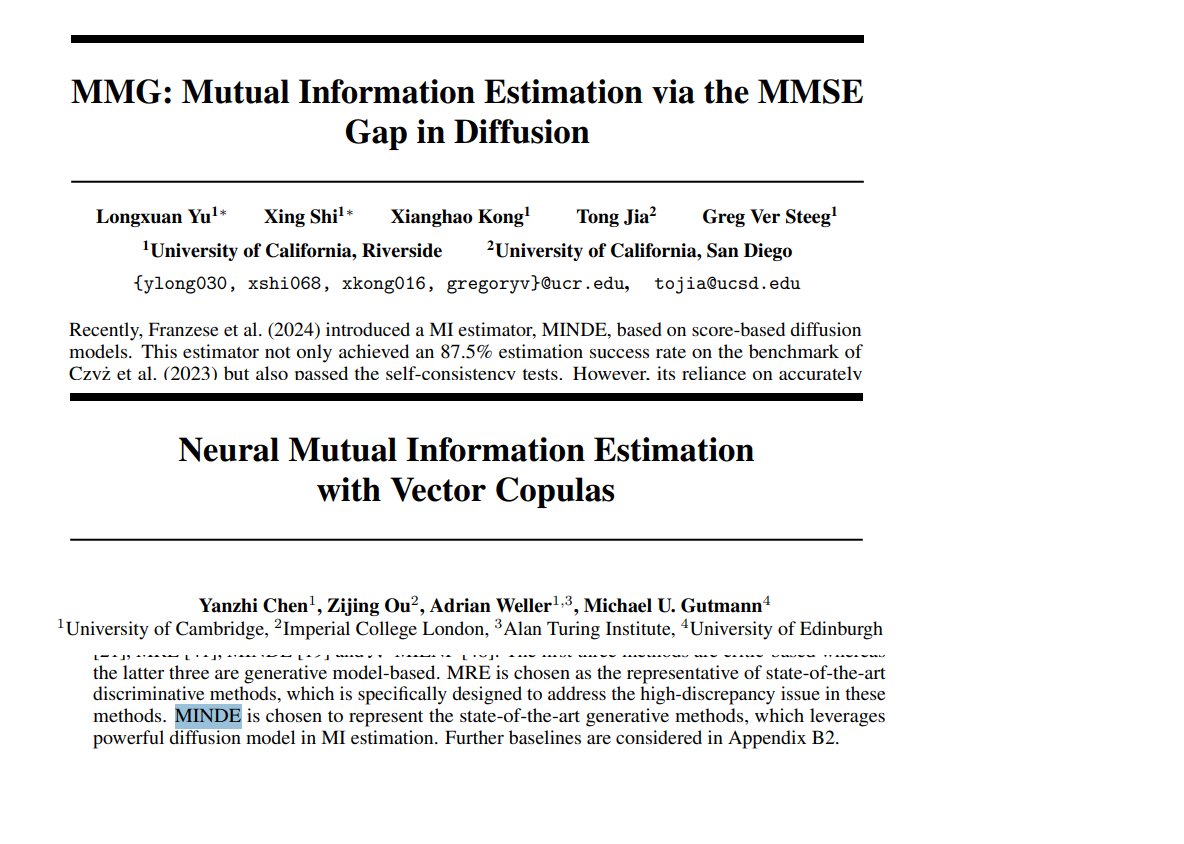
\includegraphics[width=0.9\linewidth]{figures/SotA.png}
    \label{fig:placeholder}
\end{figure}
\end{frame}

\begin{frame}{Why this gap: an intuition}
\begin{figure}
    \centering
    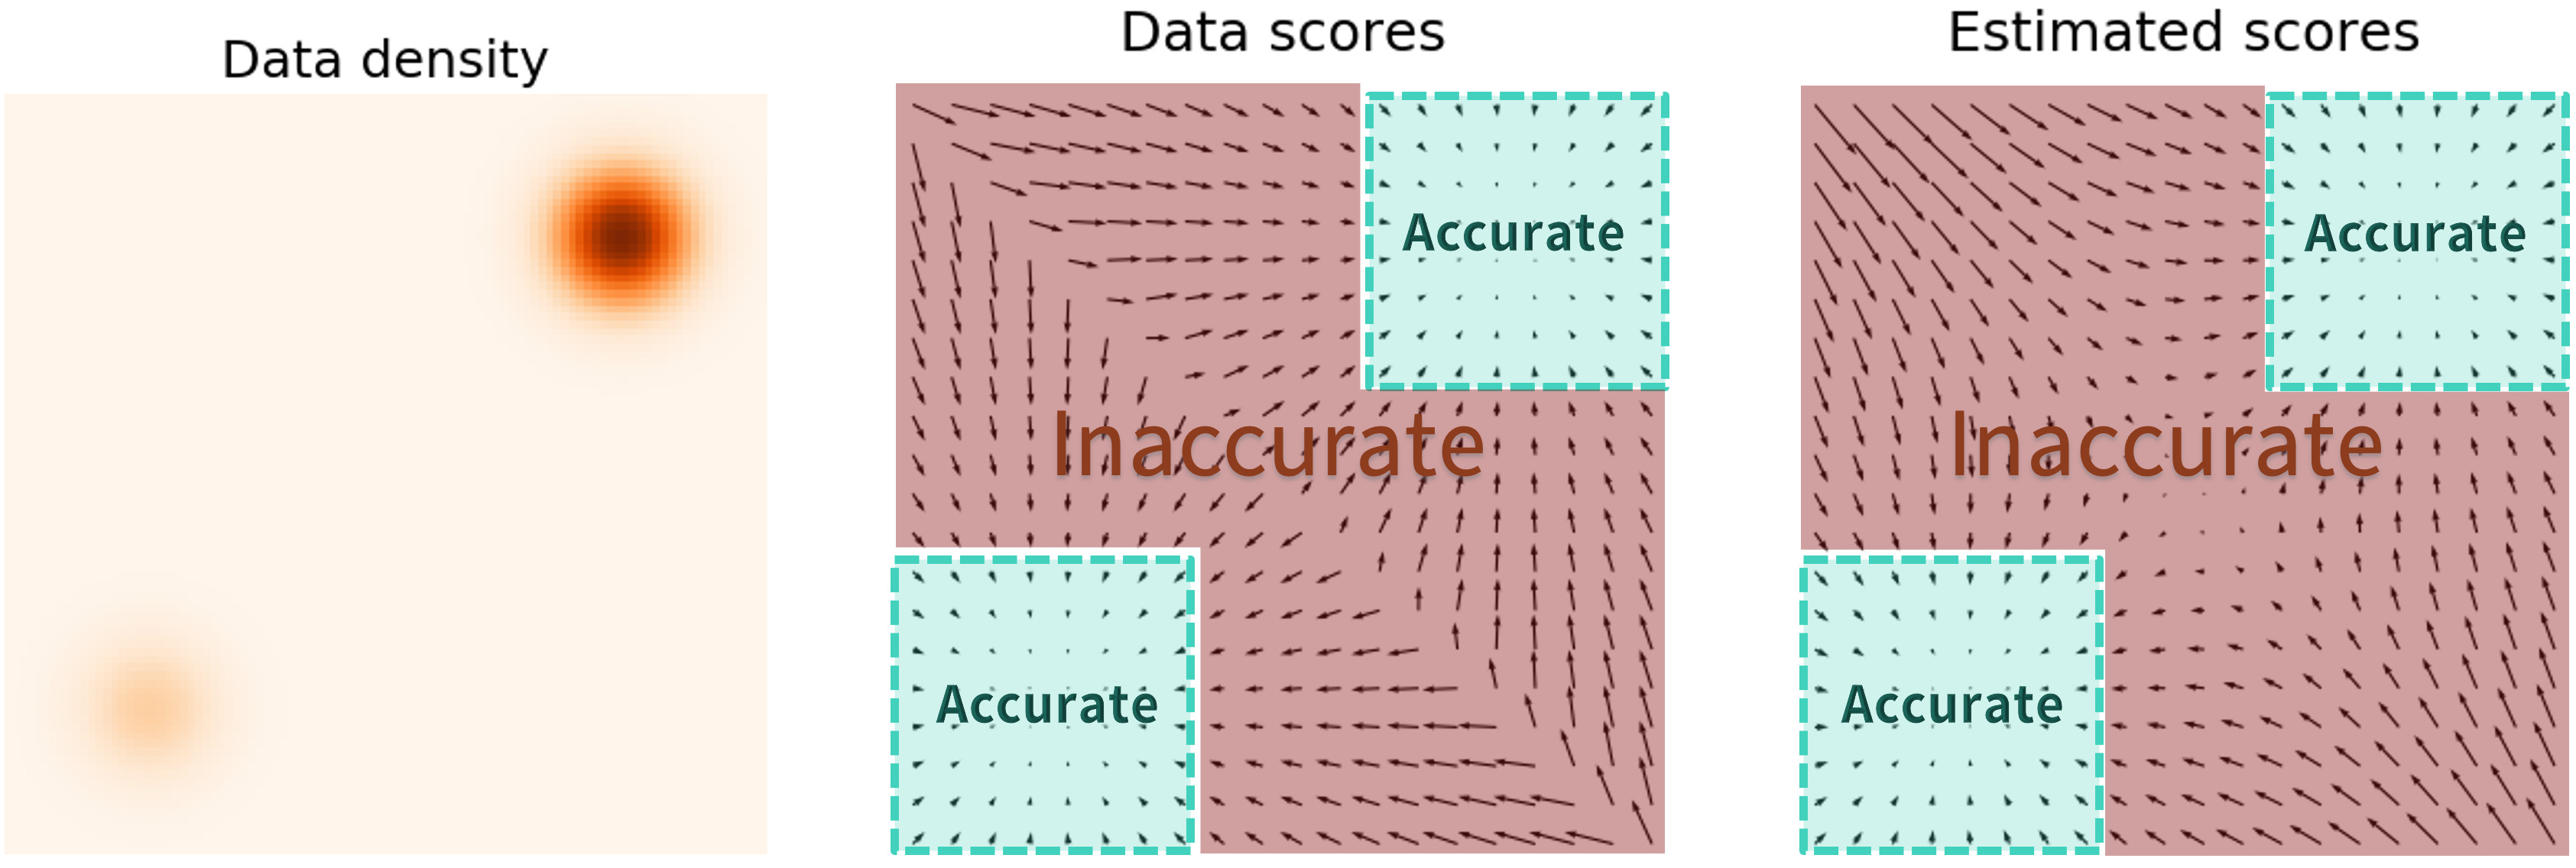
\includegraphics[width=0.5\linewidth]{figures/pitfalls.jpg}
   % \vspace*{2cm}
      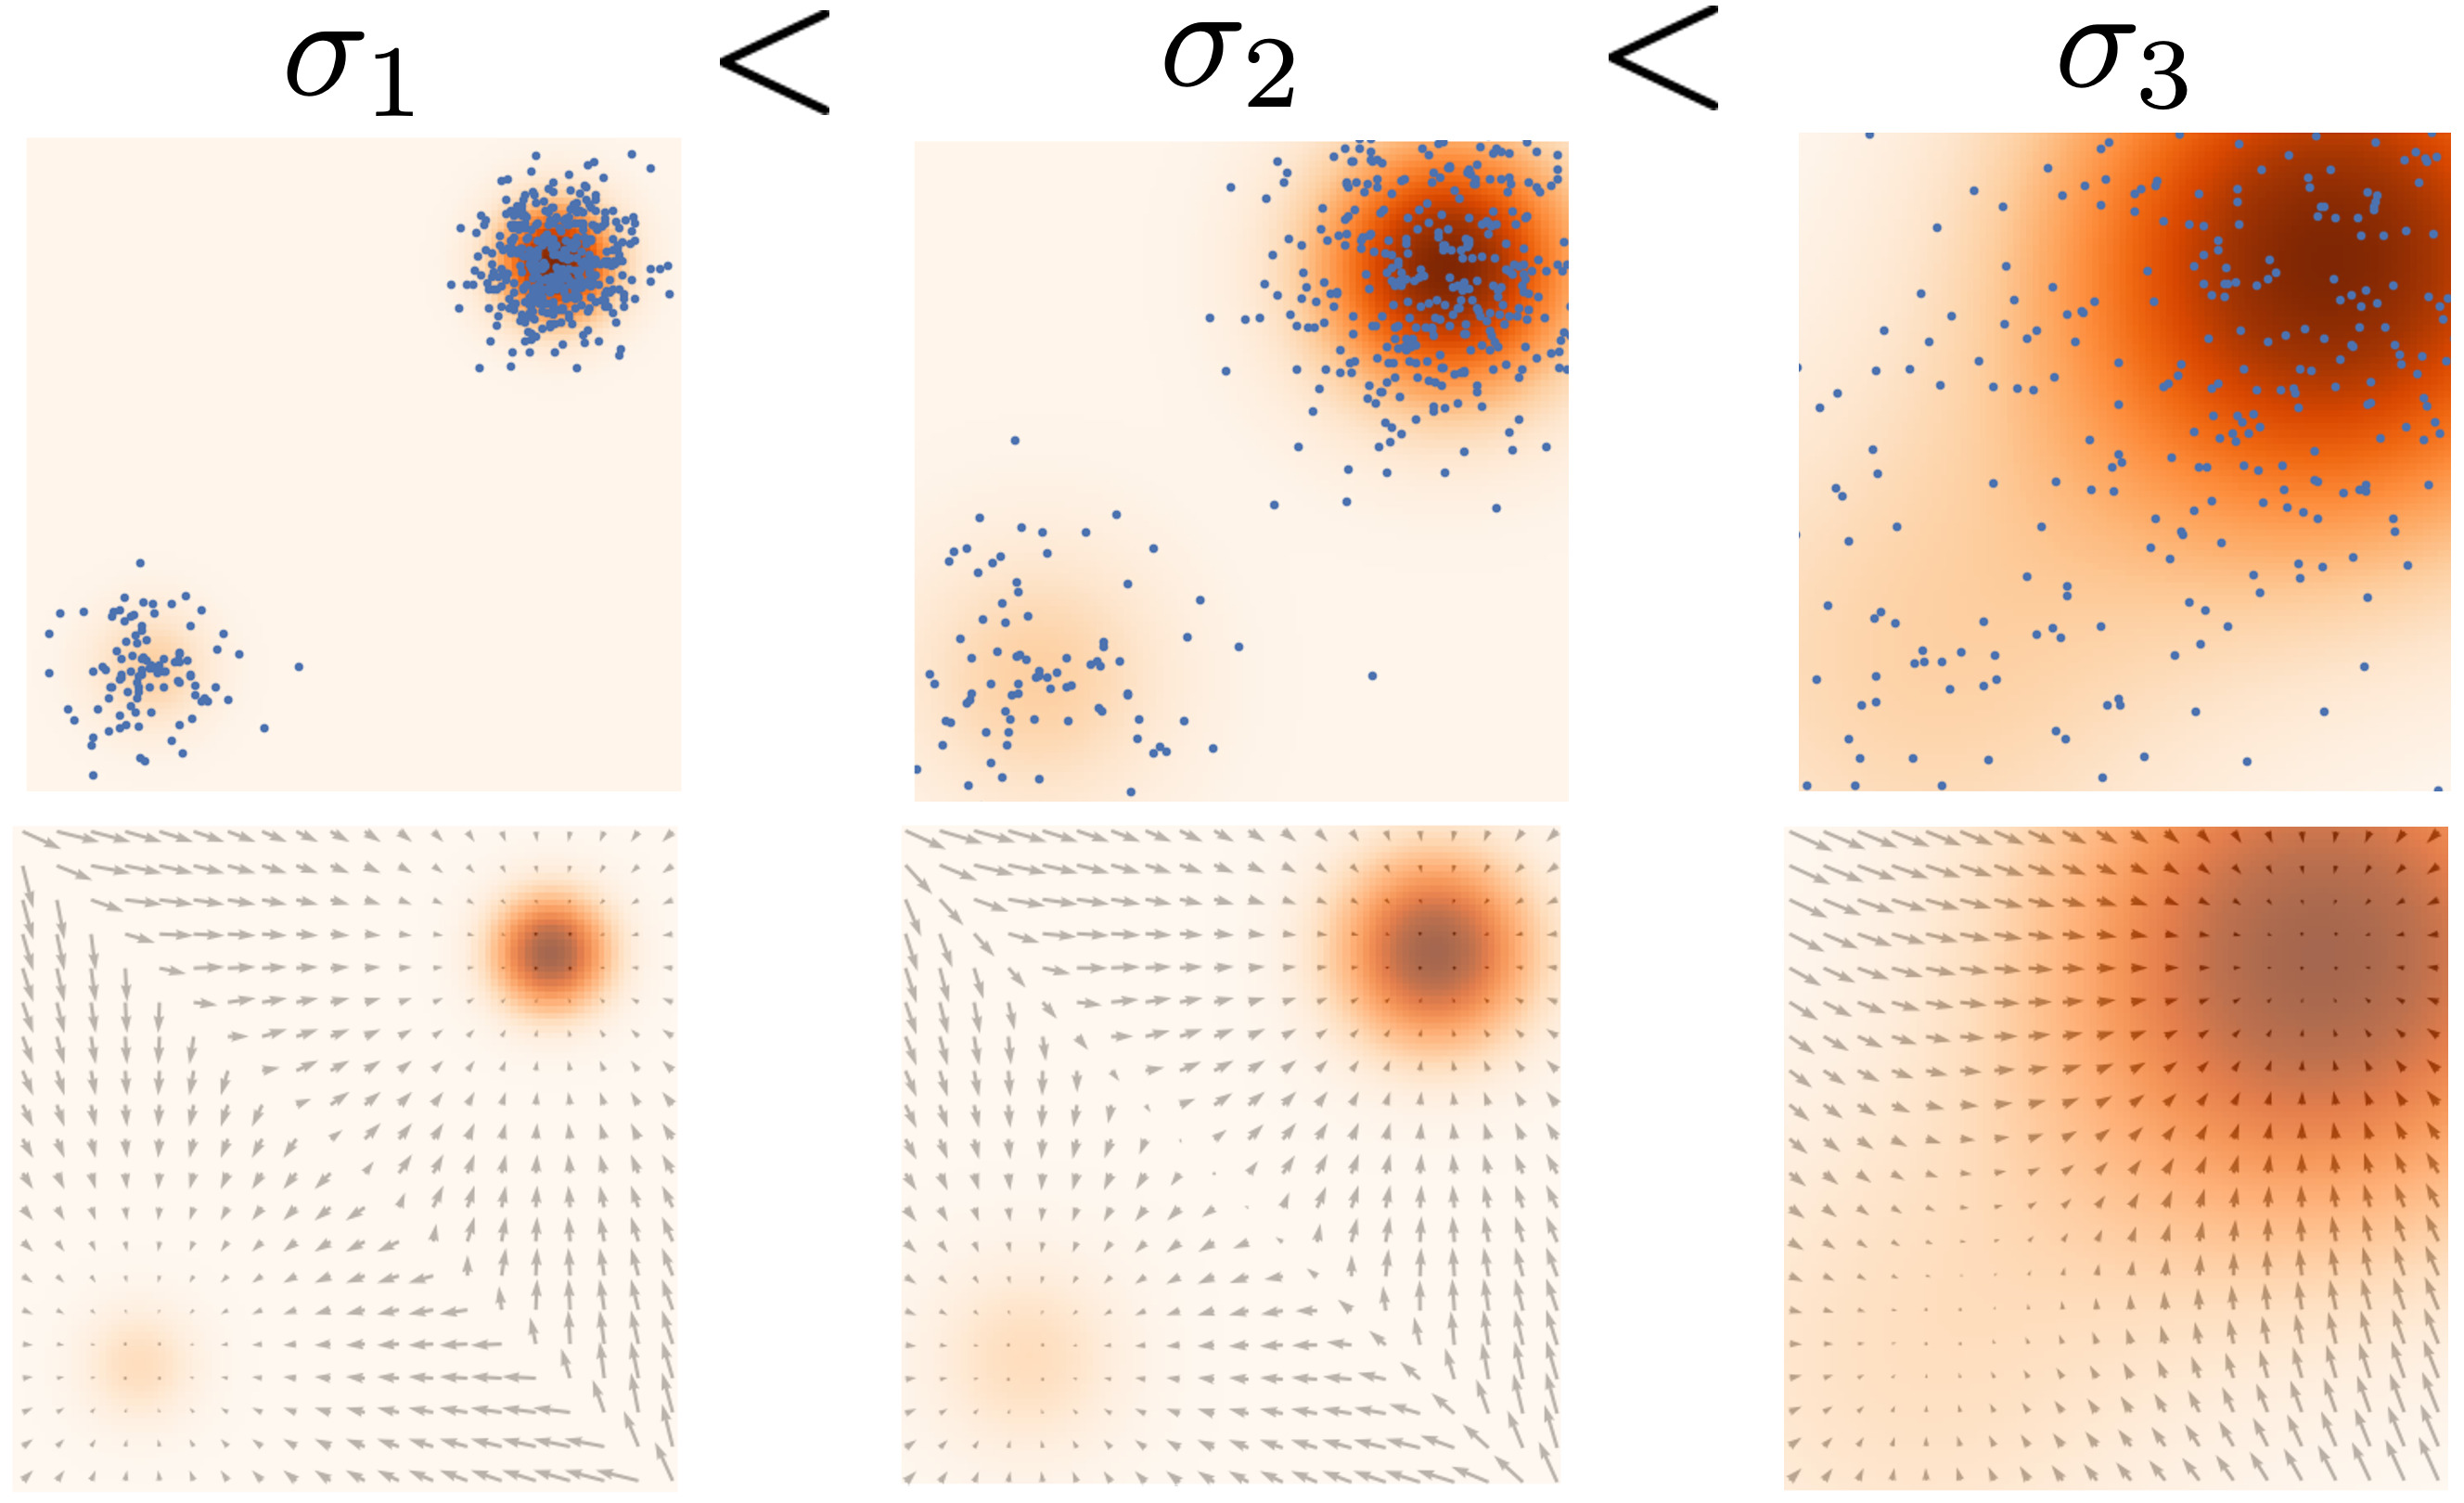
\includegraphics[width=0.5\linewidth]{figures/multi_scale.jpg}
    \caption{Credit: \url{https://yang-song.net/blog/2021/score/}}
    \label{fig:placeholder}
\end{figure}
    
\end{frame}
\begin{frame}[allowframebreaks]{Using MI to Align Text and Images }
In generative models, compute MI between images and prompts and use it as meaningful metric for alignment with human intentions!
\begin{itemize}
    \item Think of web-scale annotated datasets of image/description pairs (e.g. Laion5B, $\sim$5 billion image (1024pix res) and text pairs) as a "Telecom" channel
    \item A human sees an image and tries to convey the content of the image with a textual description.
    \item Clearly not all labelers give meaningful descriptions. The "channel capacity" depends on their skill. 
\end{itemize}

\framebreak

When you train a generative model on pairs which are not \textit{informative} enough, \textbf{alignment} suffers (def: how closely the generated data aligns with your intentions encoded via a text prompt).

What you get: top row. What you want: bottom row.
     \begin{figure}
          \centering
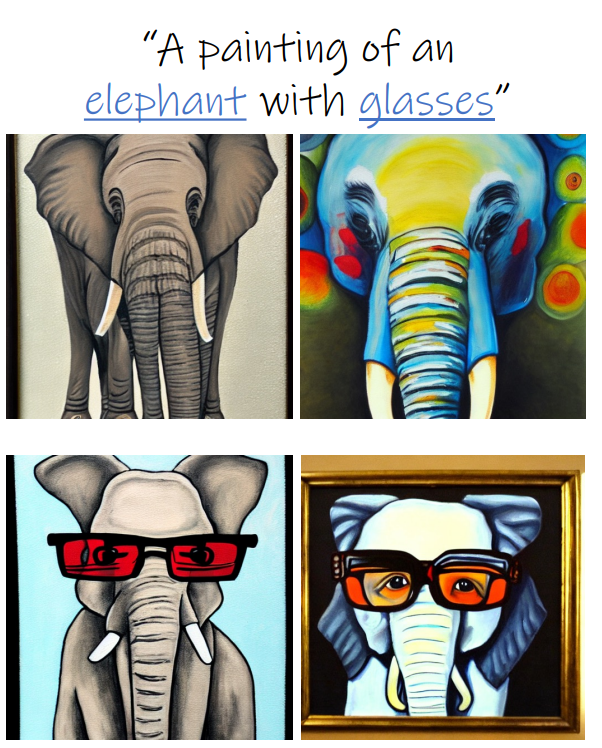
\includegraphics[scale=0.3]{figures/attexc.PNG}
      \end{figure}

Solution: use Mutual Information to select nice (sub)-distributions of texts and images, finetune existing generative models.       
\end{frame}
\begin{frame}
\begin{figure}
    \centering
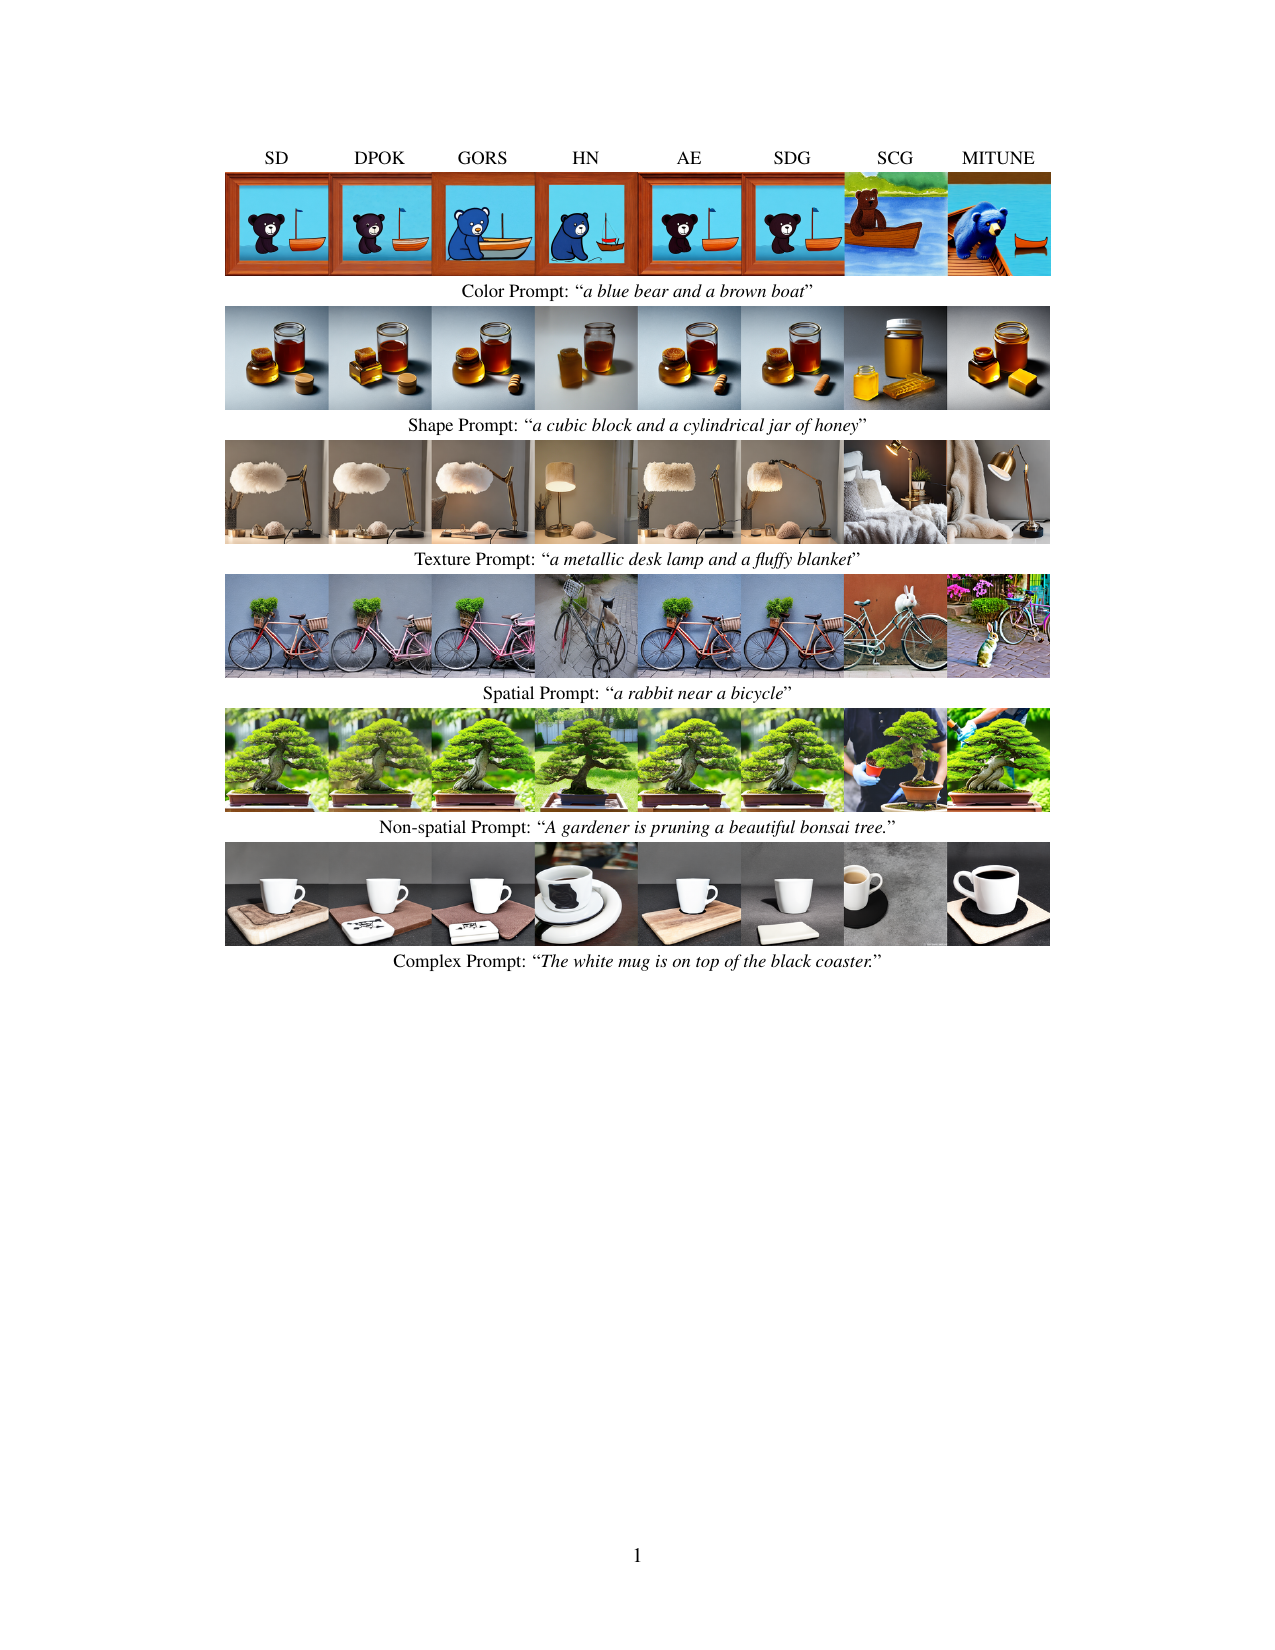
\includegraphics[scale=.5]{figures/MI_tune.pdf}
\end{figure}

Interesting open question: what is the \textit{meaning} of "MI=25.0" ?
 
\end{frame}

\section{Markov Variants}

\begin{frame}[allowframebreaks]{A different perspective}
A \textit{simpler} derivation of the estimator is based on the Feynman integration trick (a.k.a. in statistics as thermodynamic integration). Consider $p_t=\exp(t\mathcal{L})p_0,q_t=\exp(t\mathcal{L})q_0$, where $\mathcal{L}$ is the Fokker-Planck operator of a "nice" diffusion $\mathcal{L}=\nabla^\top(f\cdot)+\Delta(\cdot)$. 

Then
\begin{flalign*}
    \KL{p_0}{q_0}=\int_0^\infty \frac{\dd}{\dd t}\KL{p_t}{q_t}\dd t
\end{flalign*}
where
\begin{flalign*}
    \frac{\dd}{\dd t}\KL{p_t}{q_t}=\int \frac{\dd}{\dd t}p_t\log\frac{p_t}{q_t} +p_t \frac{\dd}{\dd t}\log\frac{p_t}{q_t} \dd x. 
\end{flalign*}
The idea of the proof: $\mathcal{L}^\dagger$ is known, integrate by parts, simplify, and obtain an expected difference of scores.
\end{frame}

\begin{frame}[allowframebreaks]{Continuous Time Markov Chains: conquering Discrete}
\begin{itemize}
    \item Consider a \textbf{discrete} random variable $A\in \chi = \left\{1,\hdots,N\right\}$ with probability measure $\mu^A$ (discrete state spaces, conflate with $p^A$)
    \item Build a CTMC in $[0,T]$ with initial conditions $\sim p^A$
    \begin{equation}\label{eq:diffsdes}
    \frac{\dd p^A_t(x)}{\dd t}=Q_t p^A_t(x)
    \end{equation}
    \item The infinitesimal generator $Q_t$ is now a matrix, whereas it was a differential operator in $\mathbb{R}^N$. Think e.g. of Queuing Theory, Epidemic Models,...
    \item We can adapt the previous calculations to this case. Then $\KL{p_0}{q_0}=$ 
\begin{equation}\label{eq:infosedd}
\mathbb{E}\left[\int_0^T\sum_{x\neq X_t} Q_{t}(X_t,x)\left(K\left(\frac{p_t(x)}{p_t(X_t)}\right)+\frac{q_t(x)}{q_t(X_t)}-\frac{p_t(x)}{p_t(X_t)}\log\frac{q_t(x)}{q_t(X_t)}\right)dt\right],
\end{equation}
where \( K(a)=a(\log(a)-1) \). $\frac{p_t(x)}{p_t(y)}$ is called the \textit{discrete score}. Again, approximated with a neural network.
\end{itemize}

\framebreak




\begin{figure}[htbp]
    \centering
    \begin{minipage}[b]{0.45\linewidth}
        \centering
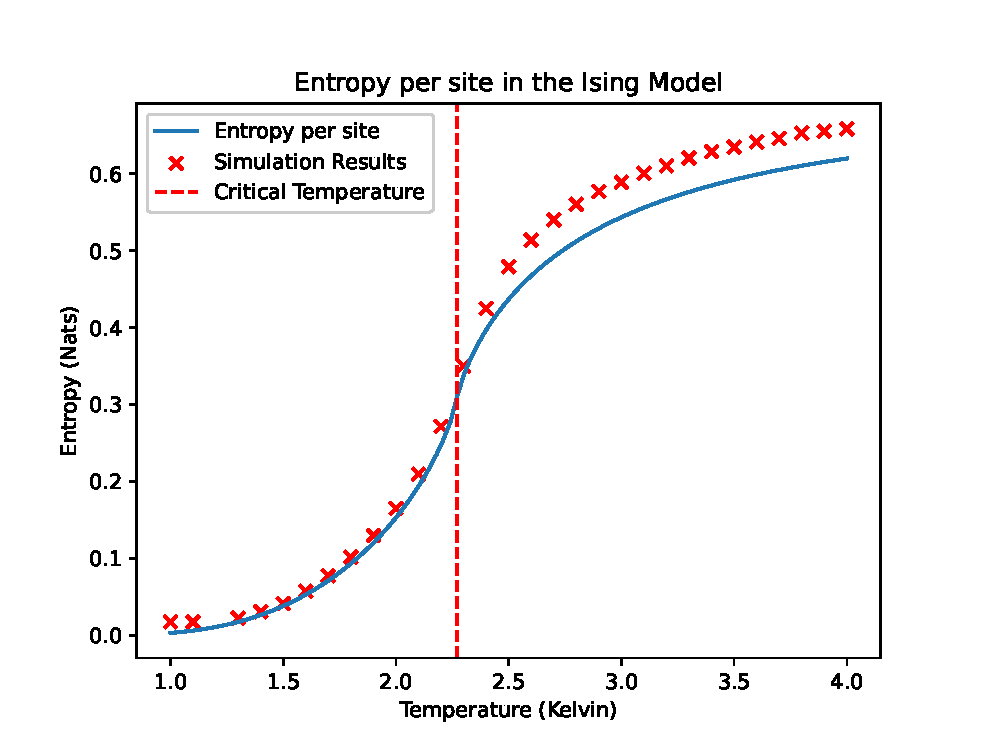
\includegraphics[width=0.75\linewidth]{figures/entropy.eps}
    \caption{Ising model entropy estimates}
\label{fig:ising}    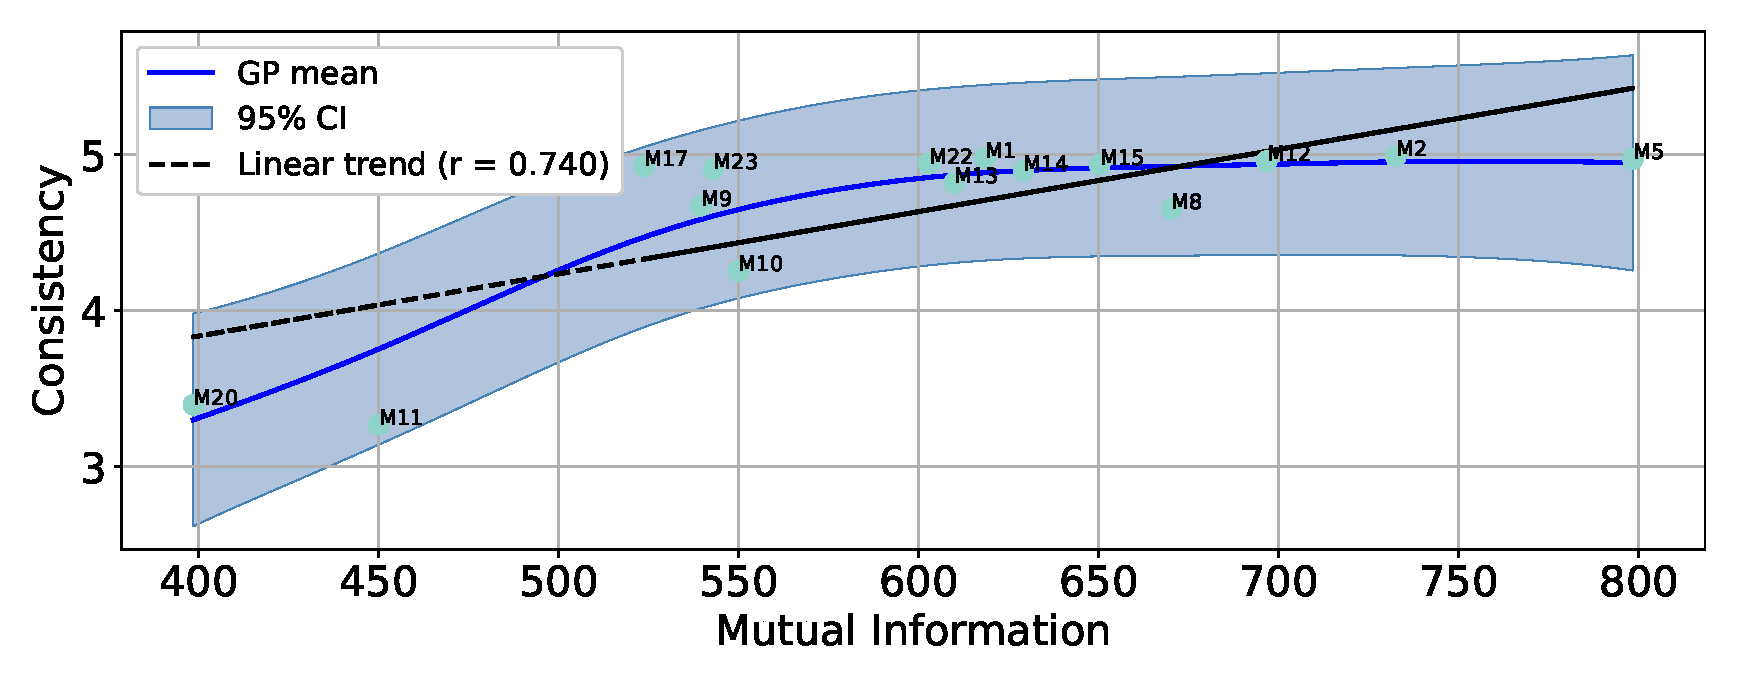
\includegraphics[width=0.75\linewidth]{figures/metric_mi_correlations_gp_consistency2_infosedd_c.eps}
    \caption{MI(summarizations,original text) vs consistency. 15 SoTA models.}
        % 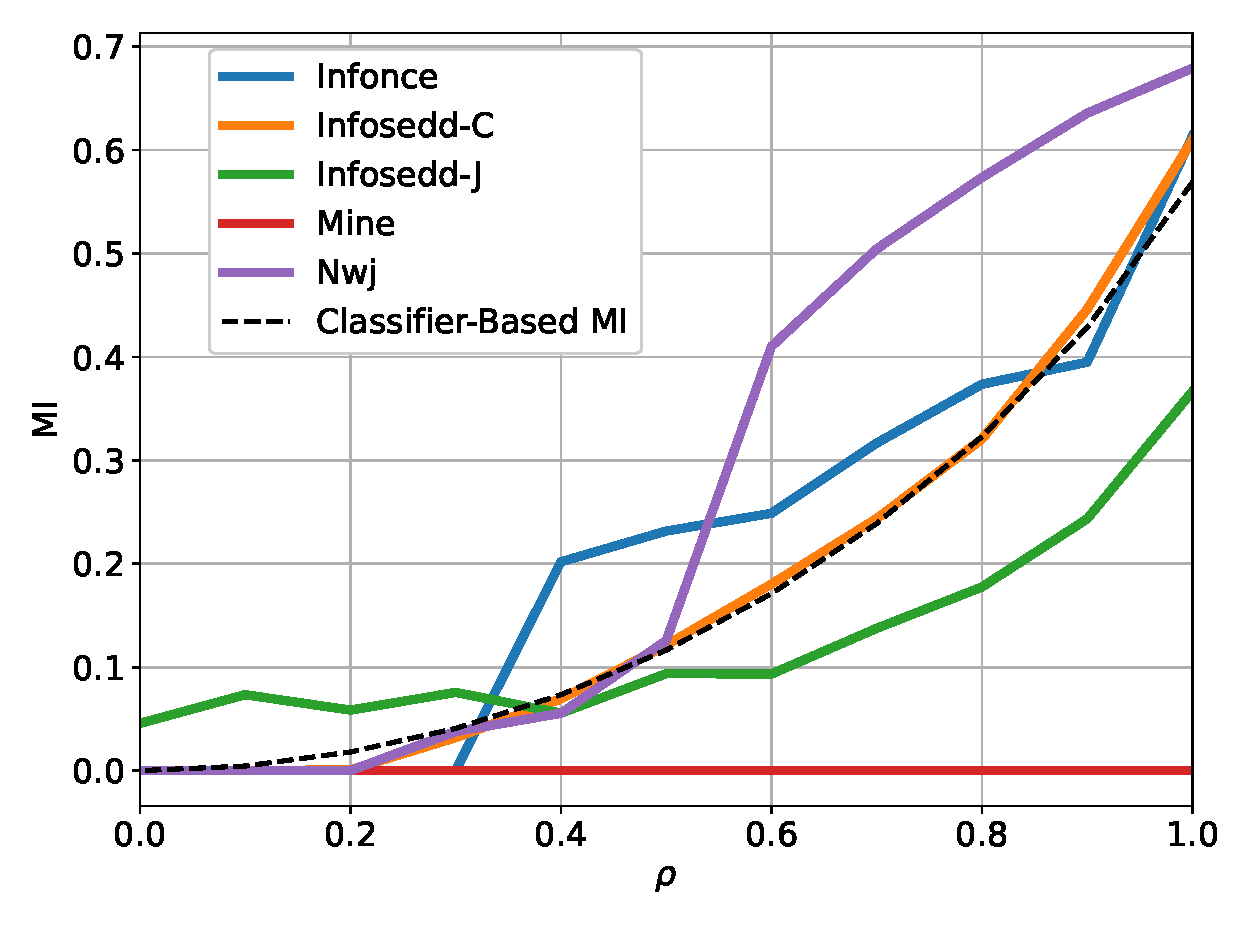
\includegraphics[width=\linewidth]{figures/consistency_dna.eps}

    \end{minipage}
    \hfill
    \begin{minipage}[b]{0.45\linewidth}
        \centering
        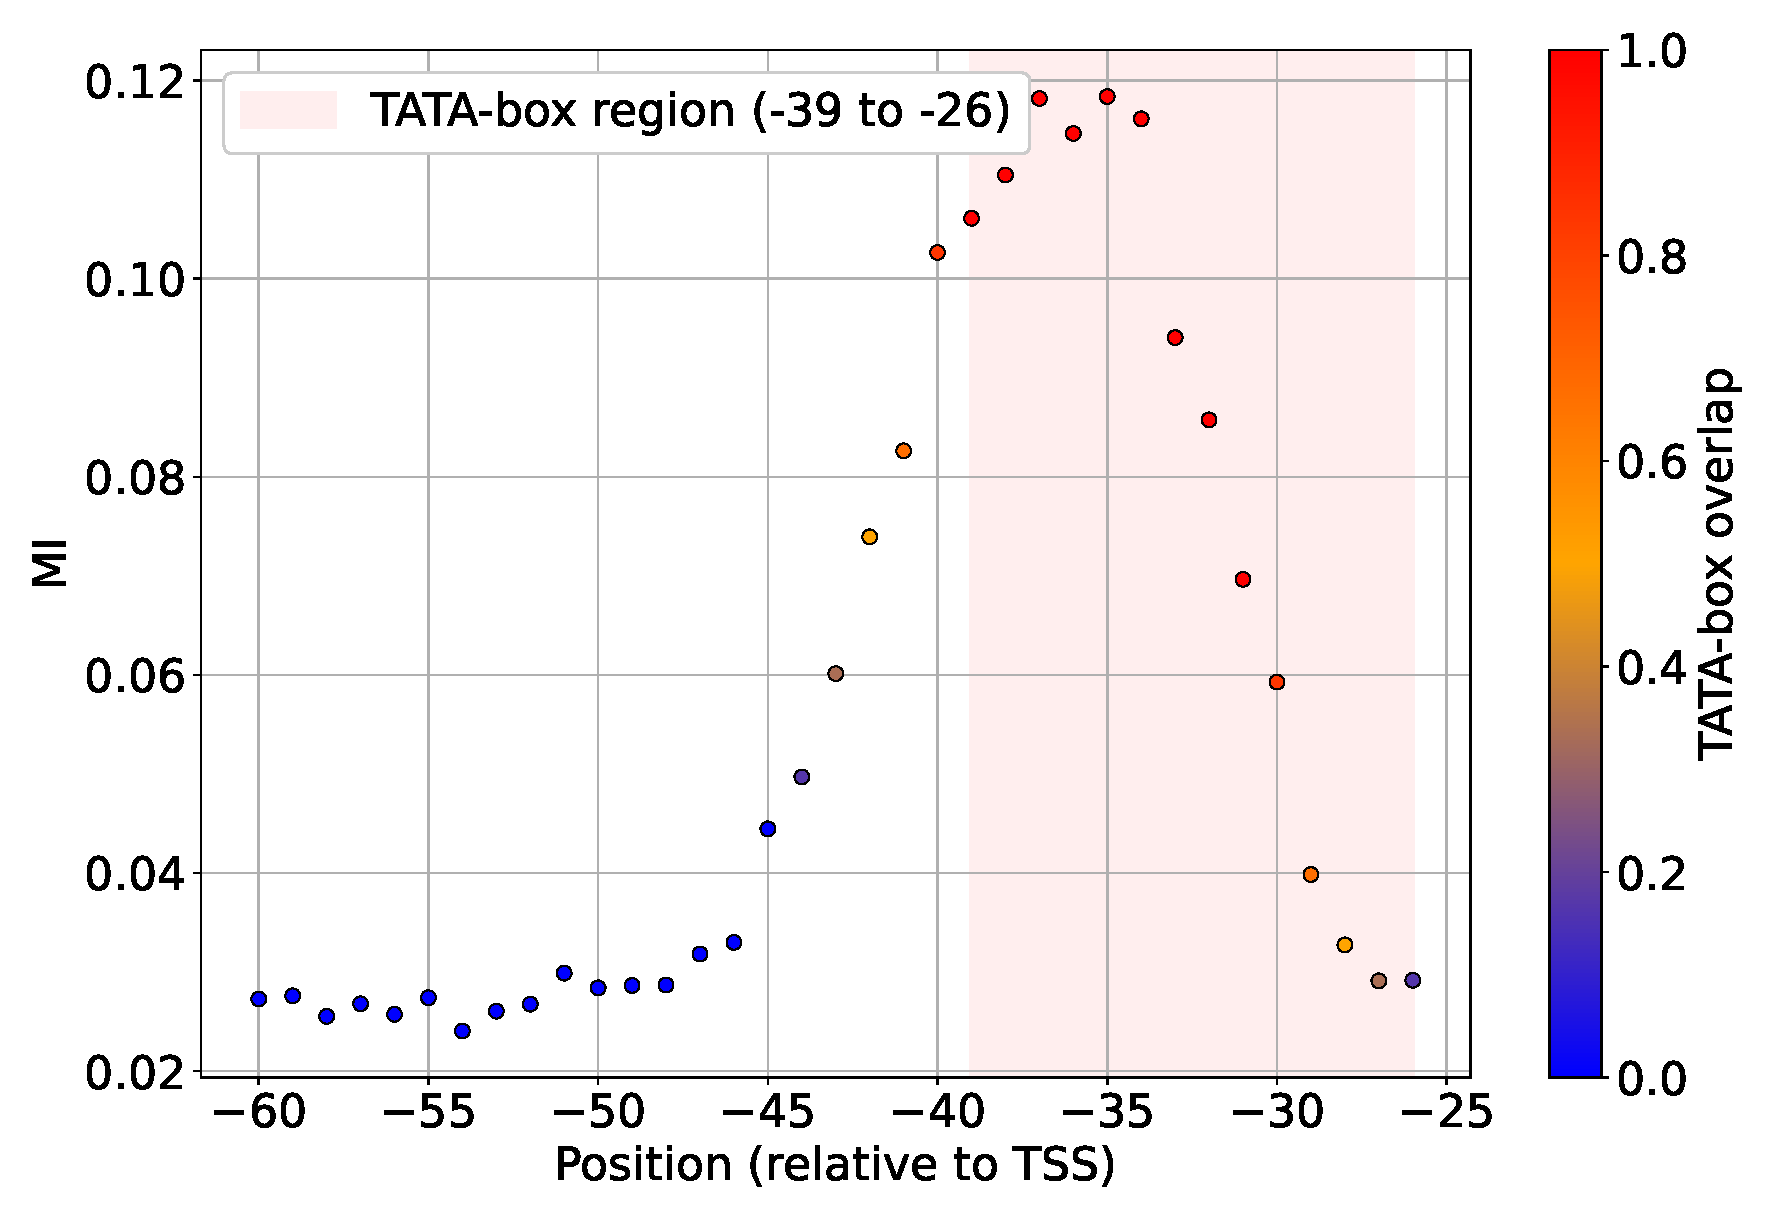
\includegraphics[width=\linewidth]{figures/tata_box_sliding_window_plot.eps}
        \caption{\textit{Arabidopsis thaliana} promoter \textsc{tata-box} identification on DNA sequences.}
        \label{fig:tata-box-search}
    \end{minipage}
\end{figure}


\end{frame}


\begin{frame}{Possible future steps}
Currently working on the infinite dimensional version (real separable Hilbert space $H$, Banach still out of reach)
\begin{equation}\label{eq:diffsde}
    \begin{cases}
    \dd X_t=\left(\mathcal{A}X_t+f(X_t,t)\right)\dd t+ \dd W_t,\\
    X_0\sim \rho_0\in P(H),%\pdata,
    \end{cases}
\end{equation}
\begin{itemize}
    \item Published among the first infinite dimensional generative models, adapting results from finite dimensions.
    \item No Lebesgue measure in infinite dimensional spaces (problem with the score function).
    \item Ergodicity is a nontrivial problem ($\rho_T$ approaches \textit{fast} something \textit{unique}).
\end{itemize}

    
\end{frame}

\section{Unpaired data matching with Mutual Information}

\begin{frame}[allowframebreaks]{Unpaired data problem}

\begin{itemize}
    \item Multimodal learning often assumes the availability of paired data.
    \item However, real-world data is frequently \textbf{unpaired across modalities}.
\end{itemize}

\begin{figure}[ht]
\centering
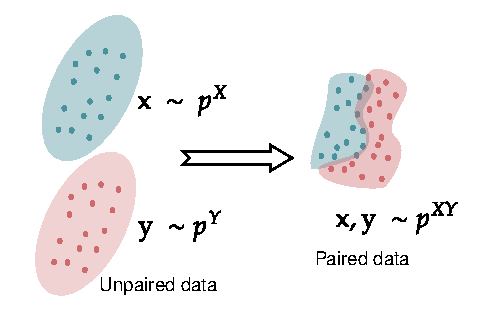
\includegraphics[width=0.5\textwidth]{figures/unpaired.pdf}
\end{figure}

%\end{block}

\framebreak

Given two marginals $\mu^{X}$ and $\mu^{Y}$,  find a joint distribution \( \mu^{XY} \) that satisfies:
\begin{itemize}
  \item The marginals constraints: \(\mu^{XY}(S\times \mathrm{R}^N)=\mu^{X}(S),\mu^{XY}( \mathrm{R}^N\times S)=\mu^{Y}(S)\)
  \item \textbf{Maximise the Mutual Information} between X and Y!
\end{itemize}

\framebreak

For example, Align ATAC and RNA measurements
\begin{figure}[h]
\centering
 \begin{subfigure}{0.42\textwidth}
        \centering
        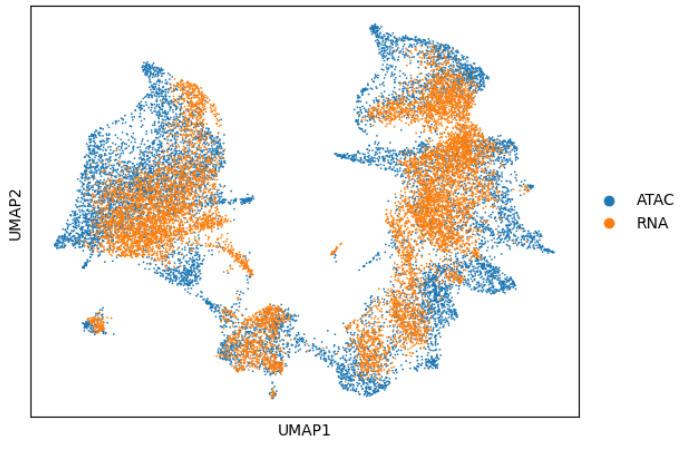
\includegraphics[width=\linewidth]{figures/gen_pbmc.png}
    \end{subfigure}
    \begin{subfigure}{0.47\textwidth}
        \centering
        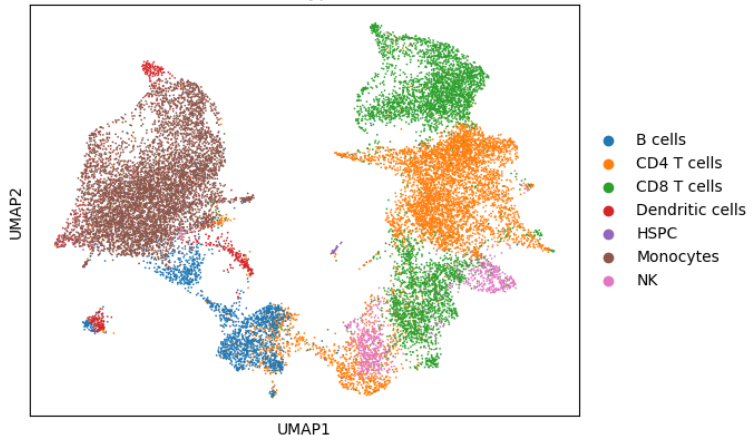
\includegraphics[width=\linewidth]{figures/out_pbmc.png}
    \end{subfigure}
    
\caption*{Conditional generation with DDMEC on PBMC.}
\label{fig:figure_pbmc}
\end{figure}

\end{frame}

\begin{frame}

Or build a machine that pairs cats and dogs without having ever seen a pairing! (Scientifically much more important that pairing RNA and ATAC)

\begin{figure}[tb]
    \centering
    \begin{subfigure}{0.11\linewidth}
        \centering
        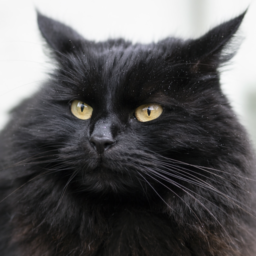
\includegraphics[width=\linewidth]{cat2dog/cond/6.png}
    \end{subfigure}
    \begin{subfigure}{0.11\linewidth}
        \centering
        
\includegraphics[width=\linewidth]{cat2dog/out/6.png}
    \end{subfigure} \hspace{2cm}
    \begin{subfigure}{0.11\linewidth}
        \centering
        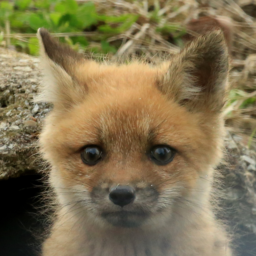
\includegraphics[width=\linewidth]{wild2dog/cond/1.png}
    \end{subfigure}
    \begin{subfigure}{0.11\linewidth}
        \centering
        
\includegraphics[width=\linewidth]{wild2dog/out/1.png}
    \end{subfigure}
    
    %%%%%%%%%%%%%%%%
     \begin{subfigure}{0.11\linewidth}
        \centering
        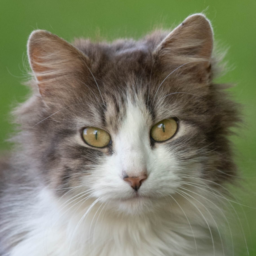
\includegraphics[width=\linewidth]{cat2dog/cond/9.png}
  
    \end{subfigure}
    \begin{subfigure}{0.11\linewidth}
        \centering
        
\includegraphics[width=\linewidth]{cat2dog/out/9.png}
    \end{subfigure}\hspace{2cm}
    \begin{subfigure}{0.11\linewidth}
        \centering
        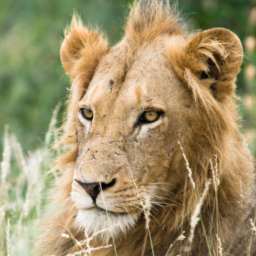
\includegraphics[width=\linewidth]{wild2dog/cond/116.png}
    \end{subfigure}
    \begin{subfigure}{0.11\linewidth}
        \centering
        
\includegraphics[width=\linewidth]{wild2dog/out/116.png}
    \end{subfigure}
%%%%%%%%%%%%%%%%%%%%%%%%%%

    \begin{subfigure}{0.11\linewidth}
        \centering
        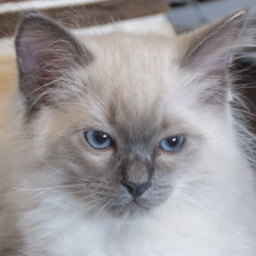
\includegraphics[width=\linewidth]{cat2dog/cond/11.png}
    \end{subfigure}
    \begin{subfigure}{0.11\linewidth}
        \centering
        
\includegraphics[width=\linewidth]{cat2dog/out/11.png}
    \end{subfigure}
    \hspace{2cm}
    \begin{subfigure}{0.11\linewidth}
        \centering
        
\includegraphics[width=\linewidth]{wild2dog/cond2/2.png}
    \end{subfigure}
    \begin{subfigure}{0.11\linewidth}
        \centering
        
\includegraphics[width=\linewidth]{wild2dog/out2/2.png}
    \end{subfigure}

     %%%%%%%%%%%%%%%%%%
\begin{subfigure}{0.11\linewidth}
        \centering
        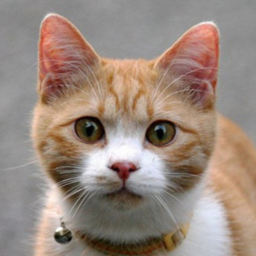
\includegraphics[width=\linewidth]{cat2dog/cond/52.png}
         \caption*{Source}
    \end{subfigure}
    \begin{subfigure}{0.11\linewidth}
        \centering
        
\includegraphics[width=\linewidth]{cat2dog/out/52.png}
           \caption*{Output}
    \end{subfigure}\hspace{2cm}
 \begin{subfigure}{0.11\linewidth}
        \centering
        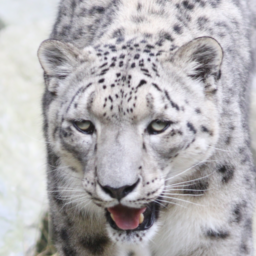
\includegraphics[width=\linewidth]{wild2dog/cond/36.png}
        \caption*{Source}
    \end{subfigure}
    \begin{subfigure}{0.11\linewidth}
        \centering
        
\includegraphics[width=\linewidth]{wild2dog/out/36.png}
        \caption*{Output}
    \end{subfigure}
    

\end{figure}
    %%%%%%%%%%%%
\end{frame}




